\documentclass{article}

% Formatting
\usepackage[utf8]{inputenc}
\usepackage[margin=1in]{geometry}
\usepackage[titletoc,title]{appendix}
\usepackage[spanish]{babel}
\usepackage{amsmath,amsfonts,amssymb,mathtools}
\usepackage{graphicx,float}
\usepackage[ruled,vlined]{algorithm2e}
\usepackage{algorithmic}
\usepackage{minted}
\usemintedstyle{borland}
\usepackage{subcaption}
\usepackage{multicol}
\usepackage{listings}
\usepackage{xcolor}
\usepackage{biblatex}
\addbibresource{ref.bib}
\usepackage{minted}



% Title content
\title{Práctica 4 Diagramas de Voronoi}
\author{Denisse Leyva}
\date{Marzo 10, 2021}

\begin{document}

\maketitle




% Introduction
\section{Introducción}
El tema de esta práctica tiene importancia en las matemáticas puras y en las ciencias aplicadas como por ejemplo la ciencia de materiales. Tomamos de un espacio bidimensional una zona con medidas conocidas que contiene $k$ puntos semillas $p_{i}$ representados por sus coordenadas $(x_{i},y_{i})$ lo que se busca es dividir esa zona en regiones llamadas celdas de Voronoi de tal forma que todos los puntos que pertenecen a la región de $p_{i}$ estén más cerca de esa semilla que de cualquier otra. \\
El modelo matemático en si es continuo, es decir, las coordenadas son números reales, pero nosotros lo vamos a discretizar en esta práctica. Se va a representar la zona por una matriz n $x$ n y las coordenadas serán entonces números enteros en $[1, n]$ \cite{Satu_Elisa_Schaeffer}.

\section{Objetivo}
Examinar de manera sistemática el efecto del número de semillas y del tamaño de la zona en la distribución de las grietas que se forman en términos de la mayor distancia manhattan entre la pieza y el exterior de la pieza \cite{Satu_Elisa_Schaeffer}.

\section{Código}
Con el siguiente código se obtiene la mayor distancia Manhattan entre la grieta y el exterior de la pieza y ser realizó un arreglo para que este dato lo tomará de diferentes tamaños de zona y con números de semilla proporcionales al tamaño de la zona. 
Se utilizaron 5 diferentes tamaños de zona (20x20, 40x40, 60x60, 80x80 y 100x100) y la cantidad de semillas se determinó por los porcentajes de longitud de zona (50\%, 75\%, 100\%, 125\%, 150\%).
El código base se obtuvo de Schaeffer \cite{Elisa_Schaeffer}. El código completo se encuentra en el repositorio \cite{Denisse_Leyva}.


\renewcommand{\listingscaption}{Código}
\begin{listing}[H]
  \begin{minted}[linenos,mathescape,texcl]{clojure}
  while True:
        g[x, y] = negro
        largo += 1
        frontera, interior = [], []
        for v in vecinos:
            (dx, dy) = v
            vx, vy = x + dx, y + dy
            if vx >= 0 and vx < n and vy >= 0 and vy < n: # existe
               if g[vx, vy] != negro: # no tiene grieta por el momento
                   if vor[vx, vy] == vor[x, y]: # misma celda
                       interior.append(v)
                   else:
                       frontera.append(v)
  \end{minted}
  \label{lst:fibo}
  \caption{Obtiene el mínimo $-$ máximo de la distancia Manhattan de la grieta.}
\end{listing}

\renewcommand{\listingscaption}{Código}
\begin{listing}[H]
  \begin{minted}[linenos,mathescape,texcl]{clojure}
 if __name__ == "__main__":
    replicas = 20
    for n in range(20, 101, 20):
        p_t = []
        porcentaje = []
        dimension = []
        for por in range(50, 151,25):
    
            profundidad = []
            k = int((por*n)/100) 
            semillas =  []
            # semillas = []
            for s in range(k):
                while True:
                    x, y = randint(0, n - 1), randint(0, n - 1)
                    if (x, y) not in semillas:
                        semillas.append((x, y))
                        break
  \end{minted}
  \label{lst:fibo}
  \caption{Representa la automatización para variar el tamaño de la zona y el número de semillas que aparecen.}
\end{listing}


\section{Resultados}

\begin{figure}[H]
\centering
\begin{subfigure}[b]{0.45\linewidth}
\includegraphics[width=\linewidth]{Grafica_dimensión_20.png}
\caption{Matriz 20x20}
\end{subfigure}
\begin{subfigure}[b]{0.45\linewidth}
\includegraphics[width=\linewidth]{Grafica_dimensión_40.png}
\caption{Matriz 40x40}
\end{subfigure}
\caption{Gráfica de distancia Manhattan vs número de semillas.}
\label{fig:westminster}
\end{figure}

\begin{figure}[H]
\centering
\begin{subfigure}[b]{0.45\linewidth}
\includegraphics[width=\linewidth]{Grafica_dimensión_60.png}
\caption{Matriz 60x60}
\end{subfigure}
\begin{subfigure}[b]{0.45\linewidth}
\includegraphics[width=\linewidth]{Grafica_dimensión_80.png}
\caption{Matriz 80x80}
\end{subfigure}
\caption{Gráfica de distancia Manhattan vs número de semillas.}
\label{fig:westminster}
\end{figure}

\begin{figure}[H]
\centering
\includegraphics[width=80mm]{Grafica_dimensión_100.png}
\caption{\label{fig3}Matriz 100x100 distancia Manhattan vs numero de semillas.}
\end{figure}

\begin{figure}[H]
\centering
\begin{subfigure}[b]{0.30\linewidth}

\includegraphics[width=\linewidth]{p4pg_20_10_2.png}
\caption{Matriz 20x20 10 semillas}
\end{subfigure}
\begin{subfigure}[b]{0.30\linewidth}

\includegraphics[width=\linewidth]{p4pg_20_30_8.png}
\caption{Matriz 20x20 30 semillas}
\end{subfigure}
\caption{Imágenes de la grieta con 10 y 30 semillas.}
\label{fig:westminster}
\end{figure}

\begin{figure}[H]
\centering
\begin{subfigure}[b]{0.30\linewidth}

\includegraphics[width=\linewidth]{p4pg_40_20_14.png}
\caption{Matriz 40x40 20 semillas}
\end{subfigure}
\begin{subfigure}[b]{0.30\linewidth}

\includegraphics[width=\linewidth]{p4pg_40_60_9.png}
\caption{Matriz 40x40 60 semillas}
\end{subfigure}
\caption{Imágenes de la grieta con 20 y 60 semillas.}
\label{fig:westminster}
\end{figure}

\begin{figure}[H]
\centering
\begin{subfigure}[b]{0.30\linewidth}

\includegraphics[width=\linewidth]{p4pg_60_30_14.png}
\caption{Matriz 60x60 30 semillas}
\end{subfigure}
\begin{subfigure}[b]{0.30\linewidth}
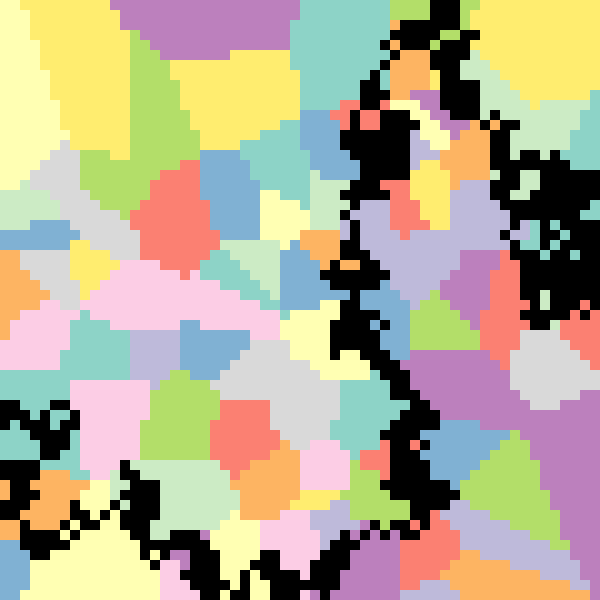
\includegraphics[width=\linewidth]{p4pg_60_90_11.png}
\caption{Matriz 60x60 90 semillas}
\end{subfigure}
\caption{Imágenes de la grieta con 30 y 90 semillas.}
\label{fig:westminster}
\end{figure}

\begin{figure}[H]
\centering
\begin{subfigure}[b]{0.30\linewidth}

\includegraphics[width=\linewidth]{p4pg_80_40_0.png}
\caption{Matriz 80x80 40 semillas}
\end{subfigure}
\begin{subfigure}[b]{0.30\linewidth}
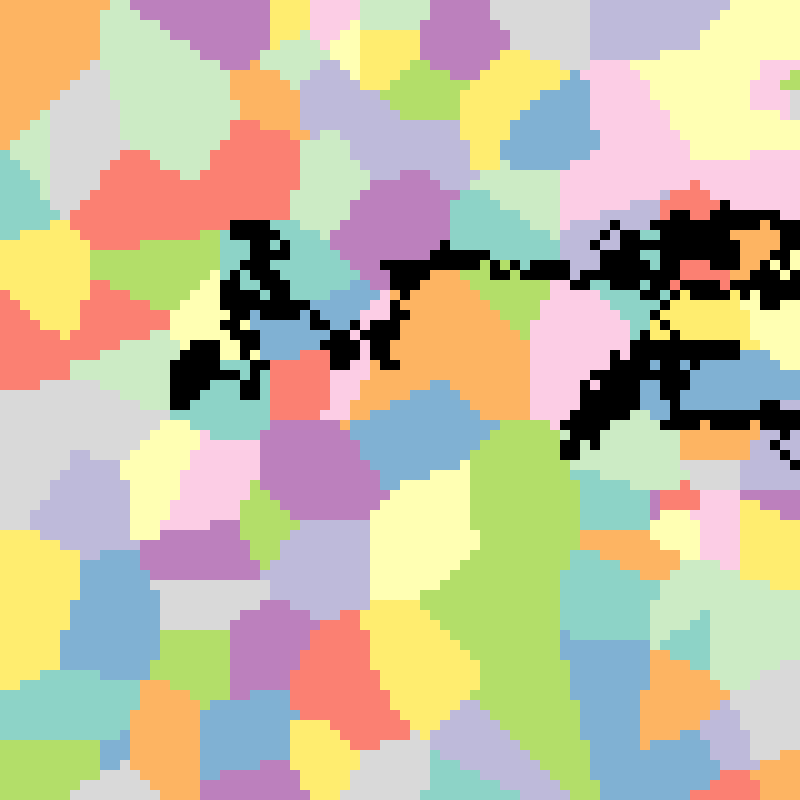
\includegraphics[width=\linewidth]{p4pg_80_120_14.png}
\caption{Matriz 80x80 120 semillas}
\end{subfigure}
\caption{Imágenes de la grieta con 40 y 120 semillas.}
\label{fig:westminster}
\end{figure}

\newpage
\section{Reto 1}
En este reto se deben hacer crecer las celdas dinámicamente alrededor de semillas de tal forma que las semillas aparezcan al azar en distintas iteraciones y crecen con una tasa exponencialmente distribuida (variable entre núcleos, pero constante para un núcleo específico) hasta toparse con las demás celdas \cite{Satu_Elisa_Schaeffer}.\\
El código completo se encuentra en el repositorio, así como el gif para poder observar el crecimiento de las semillas \cite{Denisse_Leyva}.

\renewcommand{\listingscaption}{Código}
\begin{listing}[H]
  \begin{minted}[linenos,mathescape,texcl]{clojure}
 while True:
    ac = []
    for s in range(len(semillas)):
        for pos in range(n*n):
            fil = pos // n
            col = pos % n
            if celda[fil, col] == fondo:
                ac.append(1)
            else:
                ac.append(0)
            (xs, ys) = semillas[s]
            dx, dy = fil - xs, col - ys
            dist = sqrt(dx**2 + dy**2)
            if dist <= radio[s]:
                if celda[fil, col] == fondo:
                    celda[fil, col] = ImageColor.getrgb(color[sc[s]])
        radio[s] += 1

    if semilla <= k-1:
        conteo = 0
        while True:
            if ac == []:
                ac.append(1)
            if len(sc) == k:
                break
            columna = randint(0, n - 1)
            fila = randint(0, n - 1)
            if celda[columna, fila] == fondo:
                celda[columna, fila] =  ImageColor.getrgb(color[semilla])
                sc.append(semilla)
                semillas.append((columna,fila))
                break
            if conteo == 10:
                break
            conteo += 1
    visual = zona.resize((10 * n,  10 * n), resample=Image.BOX)
    # visual.save("p4p_{:d}.png".format(ciclo))
    visual.save("p4p_{1:d}_{2:d}_{0:d}.png".format(ciclo, n, k))
    ciclo += 1
    semilla += 1
    acc = max(ac)
    if acc == 0:
        print('no hay fondo')
        break
  \end{minted}
  \label{lst:fibo}
  \caption{Representa la aparición de la semilla en diferentes iteraciones en forma radial.}
\end{listing}

\begin{figure}[H]
\centering
\begin{subfigure}[b]{0.45\linewidth}
\includegraphics[width=\linewidth]{Grafica_dimensiónr1_20.png}
\caption{Matriz 20x20}
\end{subfigure}
\begin{subfigure}[b]{0.45\linewidth}
\includegraphics[width=\linewidth]{Grafica_dimensiónr1_40.png}
\caption{Matriz 40x40}
\end{subfigure}
\caption{Gráfica de distancia Manhattan vs número de semillas.}
\label{fig:westminster}
\end{figure}

\begin{figure}[H]
\centering
\begin{subfigure}[b]{0.45\linewidth}
\includegraphics[width=\linewidth]{Grafica_dimensiónr1_60.png}
\caption{Matriz 20x20}
\end{subfigure}
\begin{subfigure}[b]{0.45\linewidth}
\includegraphics[width=\linewidth]{Grafica_dimensiónr1_80.png}
\caption{Matriz 40x40}
\end{subfigure}
\caption{Gráfica de distancia Manhattan vs número de semillas.}
\label{fig:westminster}
\end{figure}

\begin{figure}[H]
\centering
\includegraphics[width=80mm]{Grafica_dimensiónr1_100.png}
\caption{\label{fig3}Matriz 100x100 de distancia Manhattan vs número de semillas.}
\end{figure}

\begin{figure}[H]
\centering
\begin{subfigure}[b]{0.30\linewidth}

\includegraphics[width=\linewidth]{p4p_60_60_10.png}
\caption{Matriz 60x60 60 semillas iteración 10}
\end{subfigure}
\begin{subfigure}[b]{0.30\linewidth}

\includegraphics[width=\linewidth]{p4p_60_60_26.png}
\caption{Matriz 60x60 60 semillas iteración 26}
\end{subfigure}
\caption{Imágenes del comportamiento con 60 semillas con diferentes iteraciones.}
\label{fig:westminster}
\end{figure}

\begin{figure}[H]
\centering
\begin{subfigure}[b]{0.30\linewidth}

\includegraphics[width=\linewidth]{p4p_80_80_17.png}
\caption{Matriz 80x80 80 semillas iteración 17}
\end{subfigure}
\begin{subfigure}[b]{0.30\linewidth}

\includegraphics[width=\linewidth]{p4p_80_80_31.png}
\caption{Matriz 80x80 80 semillas iteración 31}
\end{subfigure}
\caption{Imágenes del comportamiento con 80 semillas con diferentes iteraciones.}
\label{fig:westminster}
\end{figure}


\begin{figure}[H]
\centering
\begin{subfigure}[b]{0.30\linewidth}

\includegraphics[width=\linewidth]{p4p_100_100_9.png}
\caption{Matriz 100x100 100 semillas iteración 9}
\end{subfigure}
\begin{subfigure}[b]{0.30\linewidth}

\includegraphics[width=\linewidth]{p4p_100_100_20.png}
\caption{Matriz 100x100 100 semillas iteración 20}
\end{subfigure}
\caption{Imágenes del comportamiento con 100 semillas con diferentes iteraciones.}
\label{fig:westminster}
\end{figure}

\begin{figure}[H]
\centering
\begin{subfigure}[b]{0.30\linewidth}

\includegraphics[width=\linewidth]{p4pg_40_40_3.png}
\caption{Matriz 40x40 40 semillas con grieta.}
\end{subfigure}
\begin{subfigure}[b]{0.30\linewidth}

\includegraphics[width=\linewidth]{p4pg_40_40_5.png}
\caption{Matriz 40x40 40 semillas con grieta.}
\end{subfigure}
\caption{Imágenes del comportamiento de la grieta con 40 semillas.}
\label{fig:westminster}
\end{figure}


\section{Reto 2}
Para este segundo reto el crecimiento ya no es determinista, sino probabilista, como para modelar fenómenos como cáncer: un núcleo propaga a vecinos desocupados con una probabilidad $p_{v}$ si un núcleo no logra crecer, se muere con una probabilidad $p_{m}$ \cite{Satu_Elisa_Schaeffer}.\\
El código completo se encuentra en el repositorio, así como el gif para poder observar el crecimiento de las semillas \cite{Denisse_Leyva}.

\renewcommand{\listingscaption}{Código}
\begin{listing}[H]
  \begin{minted}[linenos,mathescape,texcl]{clojure}
for s in range(len(semillas)):
    for pos in range(n*n):
        fil = pos //  n
        col = pos % n
        if celda[fil, col] == fondo:
            ac.append(1)
        else:
            ac.append(0)
        if vida[s] == 1:
            cic[s] = 1
            (xs, ys) = semillas[s]
            dx, dy = fil - xs, col - ys
            dist = sqrt(dx*2 + dy*2)
            if dist <= radio[s]:
                if celda[fil, col] == fondo:
                    if (random() < pv):
                        vecinos[s] += 1
                        celda[fil, col] = ImageColor.getrgb(color[sc[s]])
    v = (vecinos[s])
    radio[s] += 1
    vc = cic[s]
    if v <= 1 and cic[s] == 1 and random() < pm:        
        vida[s] = 0
        cic[s] = 2
  \end{minted}
  \label{lst:fibo}
  \caption{Determina el crecimiento probabilístico de la semilla.}
\end{listing}

\begin{figure}[H]
\centering
\begin{subfigure}[b]{0.45\linewidth}
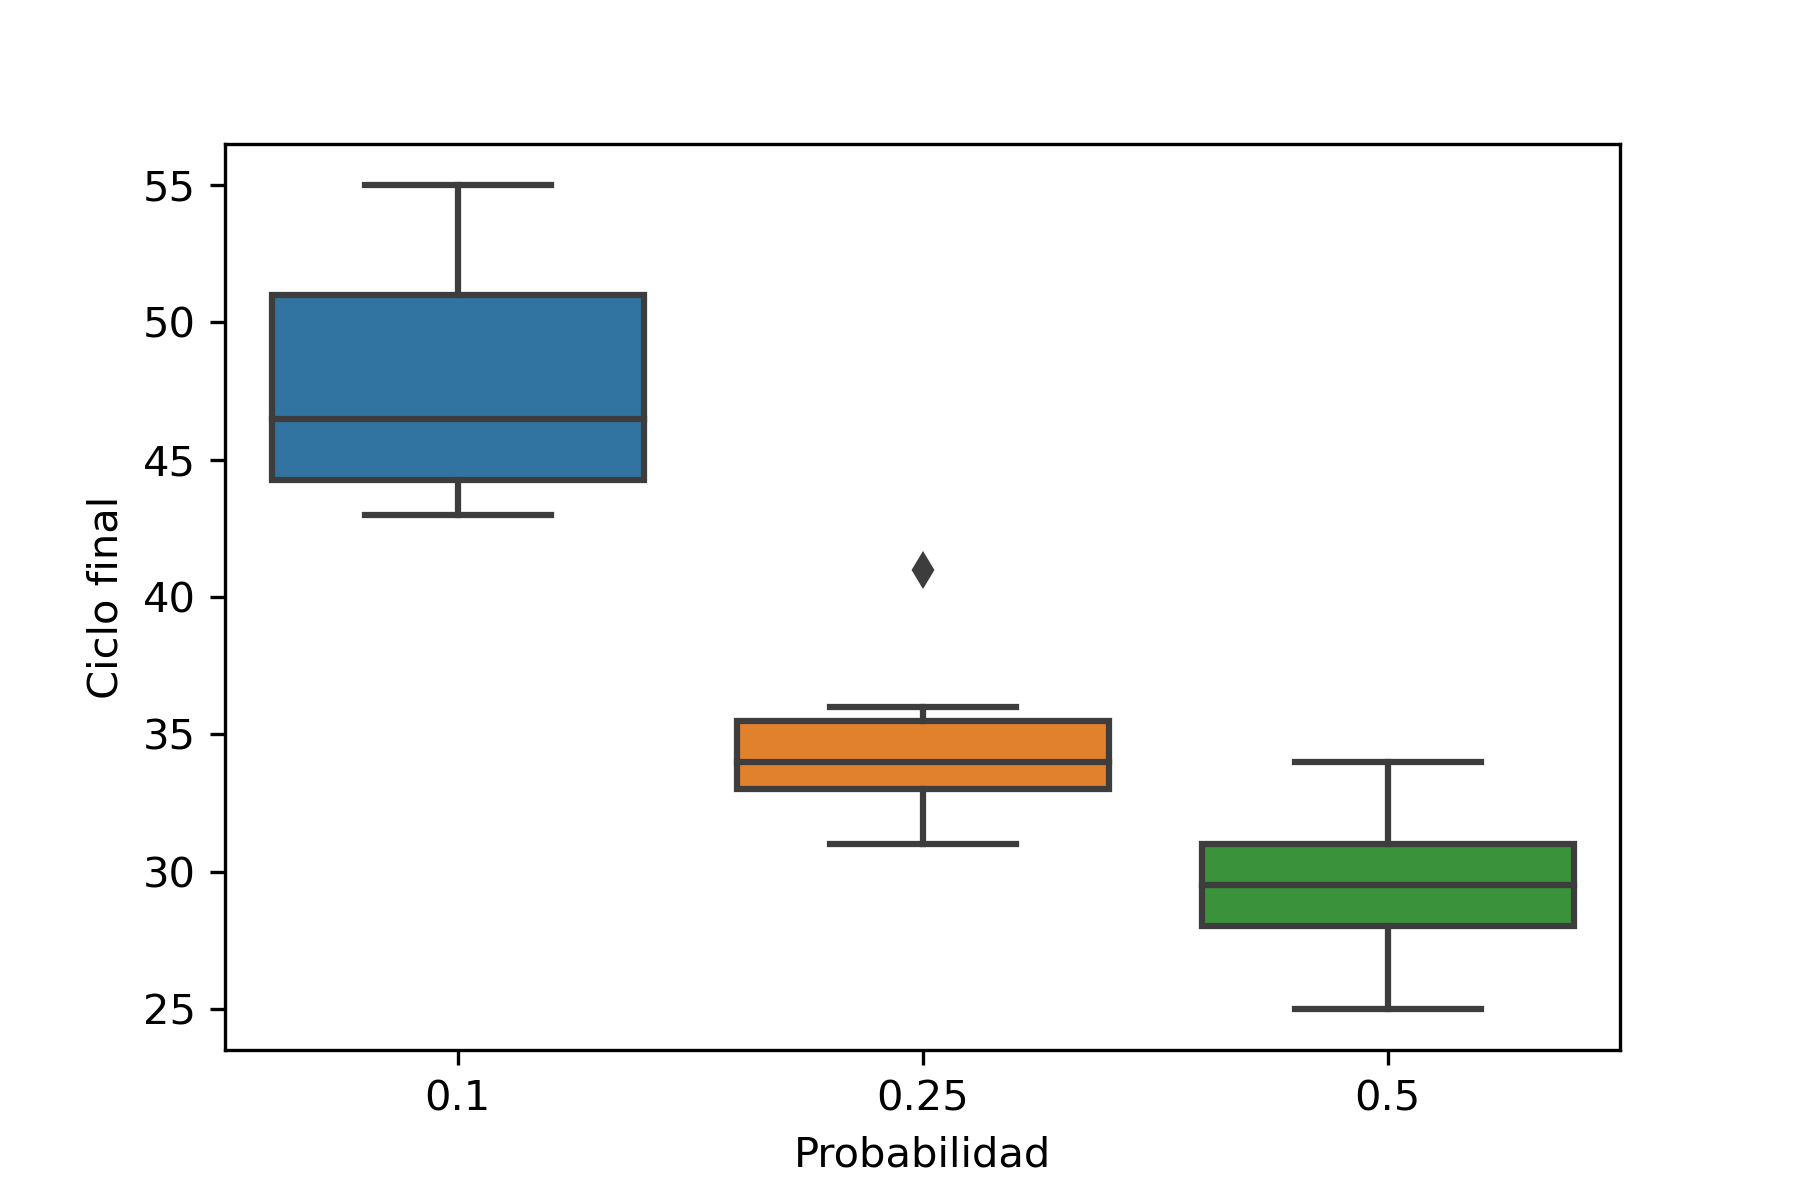
\includegraphics[width=\linewidth]{Grafica_probabilidad_25.png}
\caption{Matriz 50x50 15 semillas 25\% de que si una semilla no crece muere.}
\end{subfigure}
\begin{subfigure}[b]{0.45\linewidth}
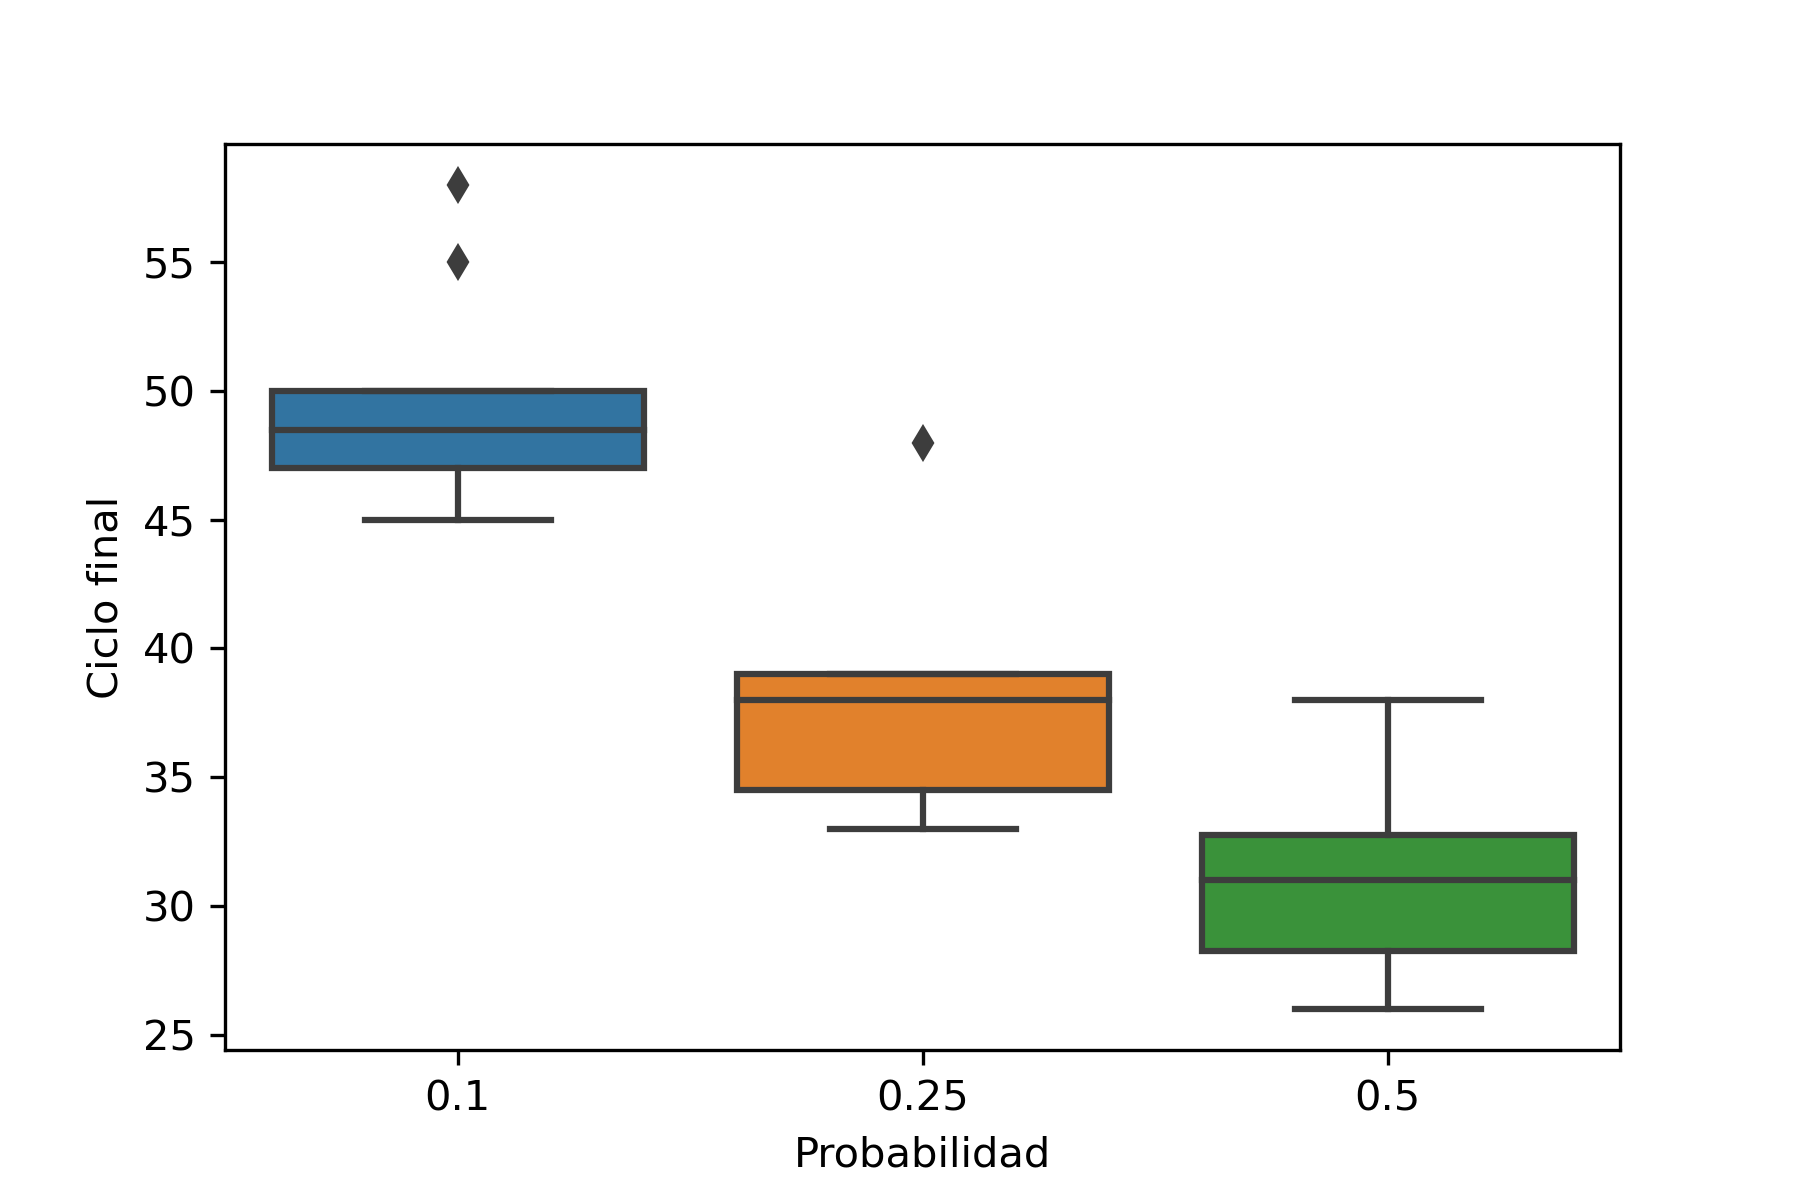
\includegraphics[width=\linewidth]{Grafica_probabilidad_50.png}
\caption{Matriz 50x50 15 semillas 50\% de que si una semilla no crece muere.}
\end{subfigure}
\caption{Gráficas de probabilidad de crecimiento de semillas.}
\label{fig:westminster}
\end{figure}

\begin{figure}[H]
\centering
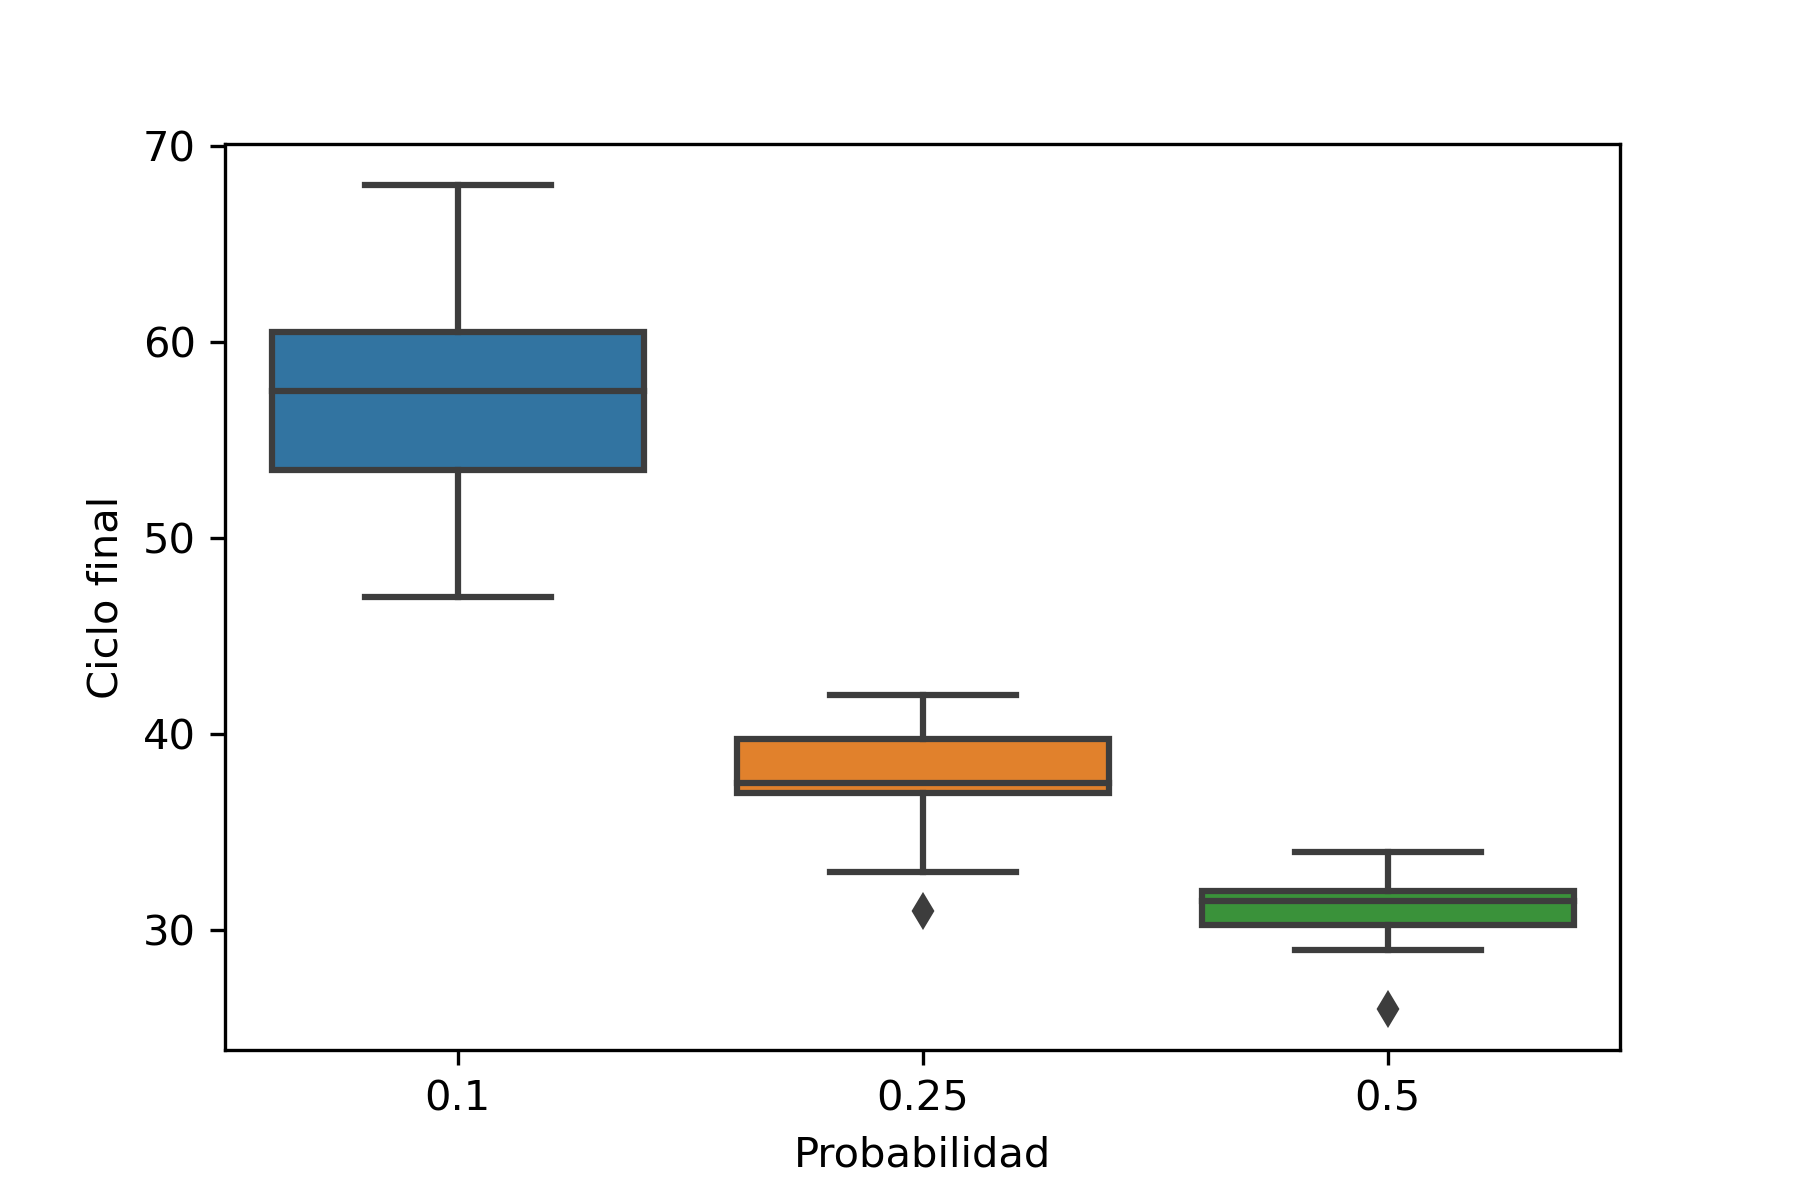
\includegraphics[width=80mm]{Grafica_probabilidad_100.png}
\caption{\label{fig3}Gráfica de probabilidad de Matriz 50x50 15 semillas con 100\% de probabilidad de que si una semilla no crece muere .}
\end{figure}

\begin{figure}[H]
\centering
\begin{subfigure}[b]{0.30\linewidth}
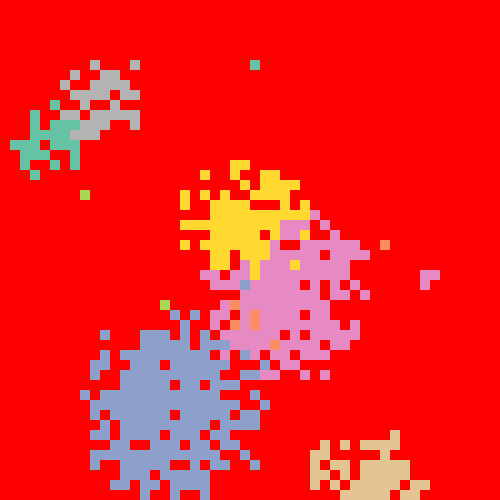
\includegraphics[width=\linewidth]{p4p_25_25_12_D.png}
\caption{Matriz 50x50 15 semillas con 25\% probabilidad de crecimiento.}
\end{subfigure}
\begin{subfigure}[b]{0.30\linewidth}
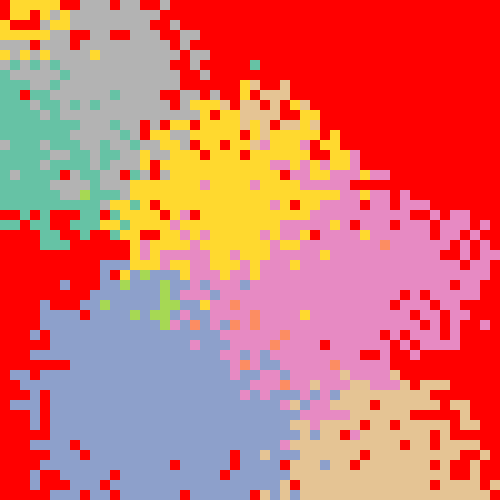
\includegraphics[width=\linewidth]{p4p_25_25_19_D.png}
\caption{Matriz 50x50 15 semillas con 25\% probabilidad de crecimiento.}
\end{subfigure}
\caption{Imágenes del comportamiento con 15 semillas en diferentes ciclos.}
\label{fig:westminster}
\end{figure}

\begin{figure}[H]
\centering
\begin{subfigure}[b]{0.30\linewidth}
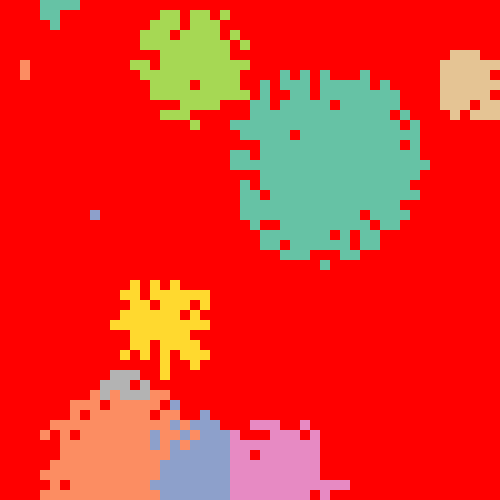
\includegraphics[width=\linewidth]{p4p_50_50_10_D.png}
\caption{Matriz 50x50 15 semillas con 50\% probabilidad de crecimiento}
\end{subfigure}
\begin{subfigure}[b]{0.30\linewidth}
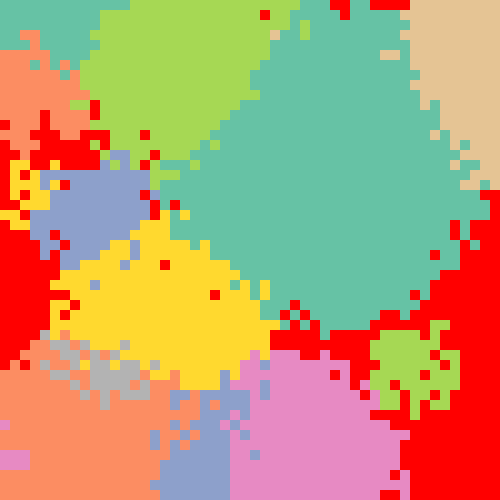
\includegraphics[width=\linewidth]{p4p_50_50_17_D.png}
\caption{Matriz 50x50 15 semillas con 50\% probabilidad de crecimiento}
\end{subfigure}
\caption{Imágenes del comportamiento con 15 semillas en diferentes ciclos.}
\label{fig:westminster}
\end{figure}

\printbibliography
\end{document}